\section{Power distribution and monitoring Module (PO)}

The PO module is composed of eight modules:

\begin{enumerate}
    \item Comp Ref Voltage (CR): provide regulated \SI{1.9}{\volt} supply rail.
    \item Precision Voltage (PV): provide regulated \SI{2.5}{\volt} supply rail.
    \item Solar Input (SI\textsubscript{1}): filter and scale solar panel output.
    \item Solar Input (SI\textsubscript{2}): filter and scale solar panel output.
    \item OR-ing (OR): combine outputs from (SI\textsubscript{1,2}).
    \item Scale V\textsubscript{batt} (SV): scale down battery voltage suitable for a \SI{2.5}{\volt} supply rail.
    \item Comparator (CO): Schmitt-Trigger with hysteresis.
    \item Master Switch (MS): control power supply of \mu M.
\end{enumerate}

\begin{figure}[h]
    \centering
    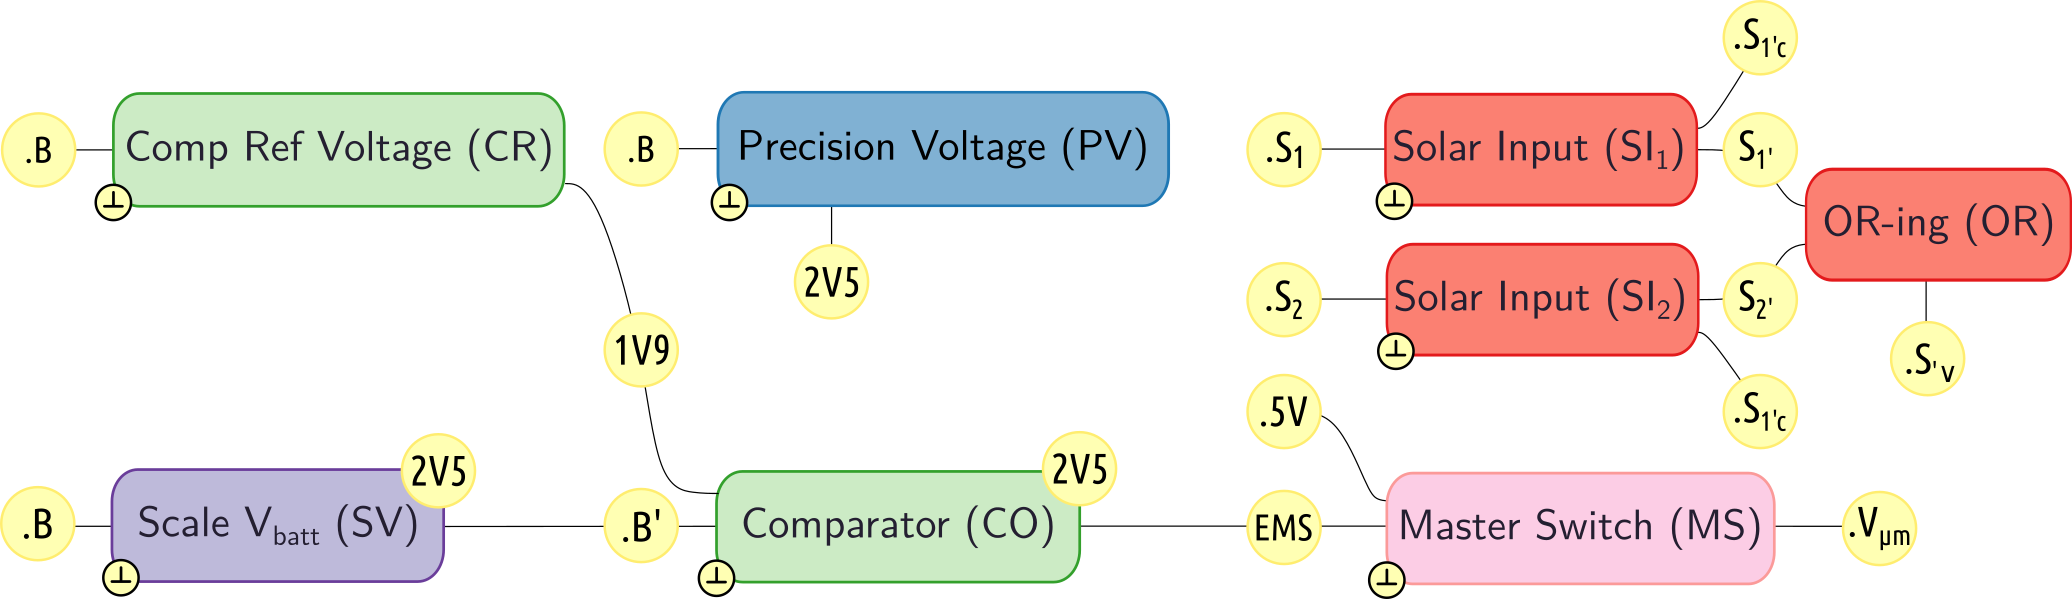
\includegraphics[width=1.0\textwidth]{PO/PO}
\end{figure}


\begin{table}[H]
    \centering
    \begin{threeparttable}[b]
        \begin{tabularx}{\linewidth}{ >{\hsize=0.15\hsize}X >
                    {\hsize=0.15\hsize}X > {\hsize=0.25\hsize}X >{\hsize=3.45\hsize}X}
            Id & Rank & Name               & Net description                                  \\
            \midrule
            1  & 1    & 1V9                & reference voltage for comparator threshold       \\
            2  & 4    & 2V5                & supply voltage for low voltage circuits\tnote{1} \\
            3  & 4    & S\textsubscript{1} & ESD protected voltage from solar panel 1         \\
            4  & 4    & S\textsubscript{2} & ESD protected voltage from solar panel 2         \\
        \end{tabularx}
        \begin{tablenotes}
            \item [1] This voltage must be lower than the minimum battery voltage.
        \end{tablenotes}
    \end{threeparttable}
    \caption{PO - NetList}
\end{table}

\clearpage

\subsection{Comp Ref Voltage Module (CR) }
\label{sec:CR}

The Comp Ref Voltage Module (CR) provides a regulated \SI{1.9}{\volt} supply rail for CO.
As we shall see later, this voltage sets the amount of hysteresis applied to the switching
threshold of the comparator.


\subsubsection{Requirements}

The reference voltage is determined by the computation shown in \ref{threshold}.


\subsubsection{Implementation}


\begin{figure}[h]
    \centering
    \includegraphics[width=0.8\textwidth]{PO/CR/CR}
    \caption{CR - schematic, from datasheet \cite{noauthor_tps783xx_2014}}
\end{figure}

\begin{table}[H]
    \centering
    \begin{threeparttable}[b]
        \begin{tabularx}{\linewidth}{ >
                    {\hsize=.25\hsize}X >
                    {\hsize=0.5\hsize}X >
                    {\hsize=.25\hsize}X  >
                    {\hsize=.5\hsize}X >
                    {\hsize=.25\hsize}X  >
                    {\hsize=3\hsize}X
            }
                  & \multicolumn{4}{c}{pin} &                                                     \\
            \cmidrule(lr){3-6}
            Id    & Net                     & Nb. & Name         & Type           & Function      \\
            \midrule
            $U_1$ & .B                      & 1   & \texttt{IN}  & \leftarrow     & input         \\
            $U_1$ & \Gnd                    & 2   & \texttt{GND} & \Gnd           &               \\
            $U_1$ & EN                      & 3   & \texttt{EN}  & \leftharpoonup & enable output \\
            $U_1$ & \Gnd                    & 4   & \texttt{GND} & \Gnd           &               \\
            $U_1$ & .1V9                    & 5   & \texttt{OUT} & \rightarrow    & output        \\
        \end{tabularx}
    \end{threeparttable}
    \caption{WD - Pin mapping}
\end{table}


\begin{table}[H]
    \centering
    \begin{threeparttable}[b]
        \begin{tabularx}{\linewidth}{
                >{\hsize=0.25\hsize}X
                >{\hsize=0.75\hsize}X
                >{\hsize=1.25\hsize}X
                >{\hsize=0.5\hsize}X
                >{\hsize=2.25\hsize}X}

            Id    & Desc                              & Order Code       & Package       & Rationale \\
            \midrule
            $U_1$ & \cite{noauthor_tps783xx_2014}     & TPS78319DDCR/922 & SOT-23-THIN-5 &           \\
            $C_1$ & \SI{1}{\micro\farad}, \SI{16}{\V} & generic          & 0603          &           \\
            $C_2$ & \SI{1}{\micro\farad}, \SI{16}{\V} & generic          & 0603          &           \\
        \end{tabularx}
    \end{threeparttable}
    % \caption{WD Module - BOM}
    \label{table:wd1}
\end{table}

\begin{table}[H]
    \centering
    \begin{threeparttable}[b]
        \begin{tabularx}{\linewidth}{ >{\hsize=.15\hsize}X >{\hsize=1.35\hsize}X >{\hsize=1.5\hsize}X }

            Id & Issue                                                       & Potential solutions                           \\
            \midrule
            1  & The choice of 1.9V is not ideal, the threshold is too high. & move the comparison function to the \mu C     \\
            1  &                                                             & use a scaling module like SV for more control \\
        \end{tabularx}
    \end{threeparttable}
    \caption{CR - issues}
\end{table}




\subsection{Precision Voltage Module (PV) }
\label{sec:PV}

The Precision Voltage Module (PV) provides a regulated \SI{2.5}{\volt} supply rail for SV and CO.


\subsubsection{Requirements}

The precision of PV has an impact on the upper threshold of CO. Given that the ambient temperature
varies between  \SI{0}{\degreeCelsius}  and  \SI{30}{\degreeCelsius} the temperature drift should be small.


\subsubsection{Implementation}


\begin{figure}[h]
    \centering
    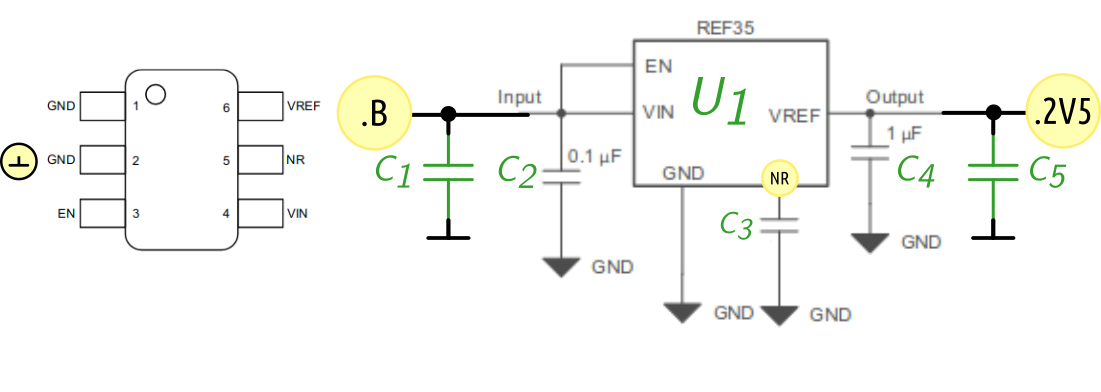
\includegraphics[width=1.0\textwidth]{PO/PV/PV}
    % \caption{CO - schematic}
\end{figure}

\begin{table}[H]
    \centering
    \begin{threeparttable}[b]
        \begin{tabularx}{\linewidth}{ >
                    {\hsize=.25\hsize}X >
                    {\hsize=0.5\hsize}X >
                    {\hsize=.25\hsize}X  >
                    {\hsize=.5\hsize}X >
                    {\hsize=.25\hsize}X  >
                    {\hsize=3\hsize}X
            }
                  & \multicolumn{4}{c}{pin} &                                                              \\
            \cmidrule(lr){3-6}
            Id    & Net                     & Nb. & Name          & Type                 & Function        \\
            \midrule
            $U_1$ & \Gnd                    & 1   & \texttt{GND}  & \Gnd                 &                 \\
            $U_1$ & \Gnd                    & 2   & \texttt{GND}  & \Gnd                 &                 \\
            $U_1$ & EN                      & 3   & \texttt{EN}   & \leftharpoonup       & enable output   \\
            $U_1$ & .B                      & 4   & \texttt{VIN}  & \leftarrow           & input           \\
            $U_1$ & NR                      & 5   & \texttt{NR}   & \leftrightsquigarrow & noise reduction \\
            $U_1$ & .2V5                    & 6   & \texttt{VREF} & \rightarrow          & output          \\
            $C_1$ & .B                      & 1   & \texttt{1}    &                      &                 \\
            $C_1$ & \Gnd                    & 2   & \texttt{2}    & \Gnd                 &                 \\
            $C_2$ & .B                      & 1   & \texttt{1}    &                      &                 \\
            $C_2$ & \Gnd                    & 2   & \texttt{2}    & \Gnd                 &                 \\
            $C_3$ & NR                      & 1   & \texttt{1}    &                      &                 \\
            $C_3$ & \Gnd                    & 2   & \texttt{2}    & \Gnd                 &                 \\
            $C_4$ & .2V5                    & 1   & \texttt{1}    &                      &                 \\
            $C_4$ & \Gnd                    & 2   & \texttt{2}    & \Gnd                 &                 \\
            $C_5$ & .2V5                    & 1   & \texttt{1}    &                      &                 \\
            $C_5$ & \Gnd                    & 2   & \texttt{2}    & \Gnd                 &                 \\
        \end{tabularx}
    \end{threeparttable}
    %\caption{WD - Pin mapping}
\end{table}

\begin{table}[H]
    \centering
    \begin{threeparttable}[b]
        \begin{tabularx}{\linewidth}{
                >{\hsize=0.25\hsize}X
                >{\hsize=0.75\hsize}X
                >{\hsize=1.25\hsize}X
                >{\hsize=0.5\hsize}X
                >{\hsize=2.25\hsize}X}
            \toprule
            Id    & Desc                               & Order Code        & Package  & Rationale \\
            \midrule
            $U_1$ & \cite{ti_ref35_2022}               & REF35250QDBVR/921 & SOT-23-6 &           \\
            $C_1$ & \SI{1}{\micro\farad}, \SI{16}{\V}  & generic           & 0603     &           \\
            $C_2$ & \SI{100}{\nano\farad}, \SI{16}{\V} & generic           & 0603     &           \\
            $C_3$ & \SI{100}{\nano\farad}, \SI{16}{\V} & generic           & 0603     &           \\
            $C_4$ & \SI{1}{\micro\farad}, \SI{16}{\V}  & generic           & 1206     &           \\
            $C_5$ & \SI{10}{\nano\farad}, \SI{16}{\V}  & generic           & 0603     &           \\
            \bottomrule
        \end{tabularx}
    \end{threeparttable}
    \caption{PV - BOM}
    \label{table:wd1}
\end{table}

\begin{table}[H]
    \centering
    \begin{threeparttable}[b]
        \begin{tabularx}{\linewidth}{ >{\hsize=.15\hsize}X >{\hsize=1.35\hsize}X >{\hsize=1.5\hsize}X }
            \toprule
            Id & Issue                                                      & Potential solutions                        \\
            \midrule
            1  & The choice of 1.9V is not ideal, the threshold is too high & move the compairison function to the \mu C \\
            \bottomrule
        \end{tabularx}
    \end{threeparttable}
    \caption{CR - issues}
\end{table}
\clearpage
\subsection{Solar Input Module (SI) }
\label{sec:SI}

The Solar Input Module (SI) filters and scales the output voltage of the solar panels.
Given the physical distance between panel and SI of approx. \SI{20}{\meter}, the inputs are susceptible
to overvoltage due to atmospheric disturbances. The solar panel output voltage should also be
digitized by \mu M.


\subsubsection{Requirements}

The voltage applied to the analog input of \mu M must not exceed \SI{3.3}{\volt}.


\subsubsection{Implementation}


\begin{figure}[h]
    \centering
    \includegraphics[width=0.5\textwidth]{PO/SI/SI}
    \caption{SI - schematic, n = 1,2}
\end{figure}

\begin{table}[H]
    \centering
    \begin{threeparttable}[b]
        \begin{tabularx}{\linewidth}{ >
                    {\hsize=.25\hsize}X >
                    {\hsize=0.5\hsize}X >
                    {\hsize=.25\hsize}X  >
                    {\hsize=.5\hsize}X >
                    {\hsize=.25\hsize}X  >
                    {\hsize=3\hsize}X
            }
                  & \multicolumn{4}{c}{pin} &                                                    \\
            \cmidrule(lr){3-6}
            Id    & Net                     & Nb. & Name       & Type                 & Function \\
            \midrule
            $D_1$ & .S\textsubscript{n'c}   & 1   & \texttt{1} & \Gnd                 &          \\
            $D_1$ & \Gnd                    & 2   & \texttt{2} & \Gnd                 &          \\
            $D_2$ & .S\textsubscript{n}     & 1   & \texttt{1} & \Gnd                 &          \\
            $D_2$ & \Gnd                    & 2   & \texttt{2} & \Gnd                 &          \\
            $D_3$ & .S\textsubscript{n}     & 1   & \texttt{A} &                      &          \\
            $D_3$ & .S\textsubscript{n'}    & 2   & \texttt{C} &                      &          \\
            $R_1$ & .S\textsubscript{n}     & 1   & \texttt{1} & \leftarrow           &          \\
            $R_1$ & .S\textsubscript{n'c}   & 2   & \texttt{2} & \leftrightsquigarrow &          \\
            $R_2$ & .S\textsubscript{n'c}   & 1   & \texttt{1} & \rightarrow          &          \\
            $R_2$ & \Gnd                    & 2   & \texttt{2} &                      &          \\
        \end{tabularx}
    \end{threeparttable}
    %\caption{WD - Pin mapping}
\end{table}

\begin{table}[H]
    \centering
    \begin{threeparttable}[b]
        \begin{tabularx}{\linewidth}{
                >{\hsize=0.25\hsize}X
                >{\hsize=0.75\hsize}X
                >{\hsize=1.25\hsize}X
                >{\hsize=0.75\hsize}X
                >{\hsize=2\hsize}X}
            \toprule
            Id    & Desc                                & Order Code         & Package  & Rationale \\
            \midrule
            $D_1$ & \cite{noauthor_cdsod323-txxsc_2019} & CDSOD323-T03SC/820 & SOD-323  &           \\
            $D_2$ & \cite{noauthor_cdsod323-txxsc_2019} & CDSOD323-T36SC/945 & SOD-323  &           \\
            $D_3$ & \cite{noauthor_cdba340l-hf_2009}    & CDBA340L-G/618     & DO-214AC &           \\
            $R_1$ & \SI{180}{\kilo\ohm}                 & generic            & 0603     &           \\
            $R_2$ & \SI{20}{\kilo\ohm}                  & generic            & 0603     &           \\
            \bottomrule
        \end{tabularx}
    \end{threeparttable}
    % \caption{WD Module - BOM}
    \label{table:wd1}
\end{table}

\begin{table}[H]
    \centering
    \begin{threeparttable}[b]
        \begin{tabularx}{\linewidth}{ >{\hsize=.15\hsize}X >{\hsize=1.35\hsize}X >{\hsize=1.5\hsize}X }
            \toprule
            Id & Issue                                & Potential solutions \\
            \midrule
            1  & reverse current of $D_3$ is too high & make further tests  \\
            \bottomrule
        \end{tabularx}
    \end{threeparttable}
    \caption{SI - issues}
\end{table}
\clearpage
\subsection{OR-ing Module (OR) }
\label{sec:OR}

The OR-ing Module (OR) combines the outputs of SI\textsubscript{1} and  SI\textsubscript{2}.


\subsubsection{Requirements}

The contribution of both panels should be summed.

\subsubsection{Implementation}

S\textsubscript{1'} and .S\textsubscript{2'} are connected.



\begin{figure}[h]
    \centering
    \includegraphics[width=0.3\textwidth]{PO/OR/OR}
    %\caption{SI - schematic, n = 1,2}
\end{figure}


\begin{table}[H]
    \centering
    \begin{threeparttable}[b]
        \begin{tabularx}{\linewidth}{ >{\hsize=.15\hsize}X >{\hsize=1.35\hsize}X >{\hsize=1.5\hsize}X }
            \toprule
            Id & Issue                                       & Potential solutions    \\
            \midrule
            1  & only one panels contributes at a given time & separate charger units \\
            \bottomrule
        \end{tabularx}
    \end{threeparttable}
    \caption{OR - issues}
\end{table}



\subsubsection{LiPo Charger}

Net \cb{net}{.S\textsubscript{'\lor}} is connected to \texttt{SOLAR IN +} of the charger shown in Fig.\ref{fig:wv}.

\begin{figure}[h]
    \centering
    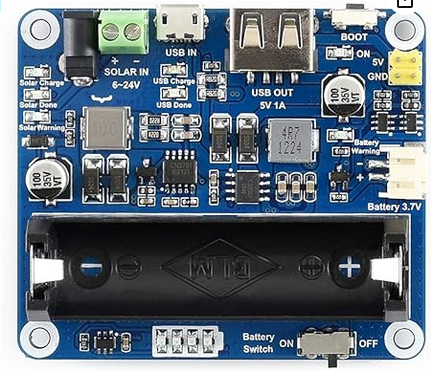
\includegraphics[scale=0.4]{charger}
    \caption{Waveshare solar power LiPo charger}
    \label{fig:wv}
\end{figure}
\clearpage
\subsection{Scale V\textsubscript{batt}  Module (SV) }
\label{sec:SV}

The Scale V\textsubscript{batt} Module (SV) scales the battery voltage to make it compatible with
the operation voltage of  \mu M (\SI{3.3}{\volt}).


\subsubsection{Requirements}

The battery voltage  \cb{net}{.B} must be scaled such that the maximum value is close to
the upper input voltage limit of SV.
We suppose that the maximum voltage of a one-cell LiPo battery does not exceed  \SI{4.1}{\V}.
Let us recall that SV must operate from \SI{2.5}{\volt} which is lower than the minimum battery voltage.
There is some debate on how low LiPo batteries can be discharged. Some argue that \SI{2.5}{\V}
can be set a lower threshold. We have decided to not got beyond \SI{3}{\V}
until we have carried out our own measurements with our
batteries.



\subsubsection{Implementation}
\label{sss:svi}

We choose $U_1$ with an input common mode range of \SI{\pm100}{\milli\volt} beyond rail.
That means we can map the maximum battery voltage
to the supply rail of the op amp (\SI{2.5}{\volt}) while still keeping some margin. \par


The scale coefficient is thus $k = \frac{\si{2.5}{V}}{\si{4.1}{V}} = 0.61$.
I choose $R_1 = \SI{129}{\kilo\ohm}, R_1 = \SI{200}{\kilo\ohm}, k = 0.645$.
The maximum voltage at the non-inverting input of the buffer is therefore
$V_{max} = 0.645 \cdot\SI{4.1}{\V}  = \SI{2.64}{\V}$.

\par

\begin{figure}[h]
    \centering
    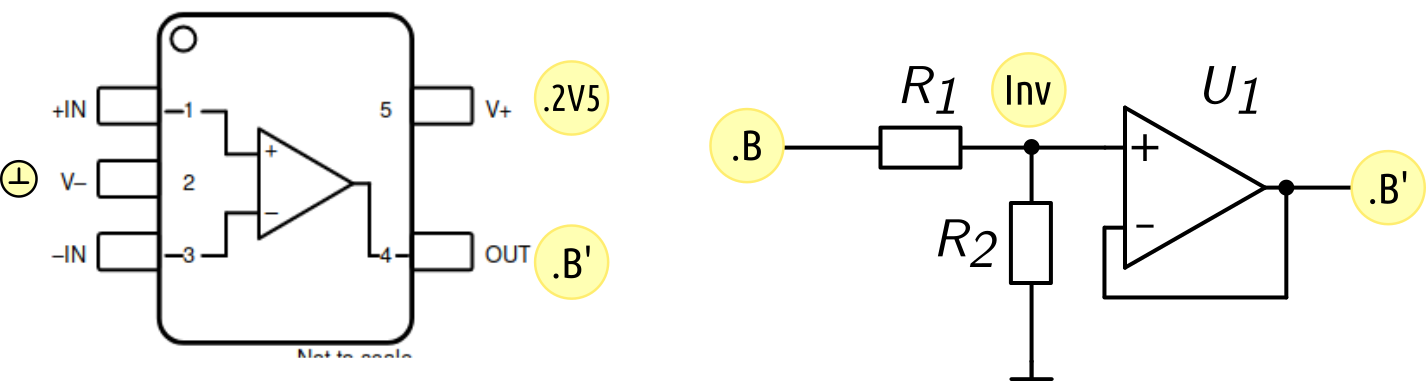
\includegraphics[width=1.0\textwidth]{PO/SV/SV}
    % \caption{SI - schematic, n = 1,2}
\end{figure}
\begin{table}[H]
    \centering
    \begin{threeparttable}[b]
        \begin{tabularx}{\linewidth}{ >
                    {\hsize=.25\hsize}X >
                    {\hsize=0.5\hsize}X >
                    {\hsize=.25\hsize}X  >
                    {\hsize=.5\hsize}X >
                    {\hsize=.25\hsize}X  >
                    {\hsize=3\hsize}X
            }
                  & \multicolumn{4}{c}{pin} &                                                         \\
            \cmidrule(lr){3-6}
            Id    & Net                     & Nb. & Name         & Type             & Function        \\
            \midrule
            $U_1$ & Inv                     & 1   & \texttt{+IN} & \leftsquigarrow  & input           \\
            $U_1$ & \Gnd                    & 2   & \texttt{V-}  & \Gnd             &                 \\
            $U_1$ & .B'                     & 3   & \texttt{-IN} & \leftsquigarrow  & inverting input \\
            $U_1$ & .B'                     & 4   & \texttt{OUT} & \rightsquigarrow & output          \\
            $U_1$ & .2V5                    & 5   & \texttt{V+}  & \leftarrow       & power supply    \\
            $R_1$ & .B                      & 1   & \texttt{OUT} &                  &                 \\
            $R_1$ & Inv                     & 2   & \texttt{OUT} &                  &                 \\
            $R_2$ & Inv                     & 1   & \texttt{OUT} &                  &                 \\
            $R_2$ & \Gnd                    & 2   & \texttt{OUT} &                  &                 \\
        \end{tabularx}
    \end{threeparttable}
    %  \caption{WD - Pin mapping}
\end{table}

\begin{table}[H]
    \centering
    \begin{threeparttable}[b]
        \begin{tabularx}{\linewidth}{
                >{\hsize=0.25\hsize}X
                >{\hsize=0.75\hsize}X
                >{\hsize=1.5\hsize}X
                >{\hsize=0.5\hsize}X
                >{\hsize=2\hsize}X}
            \toprule
            Id    & Desc                       & Order Code           & Package & Note                                           \\
            \midrule
            $U_1$ & \cite{ti_opax391_2022}     & OPA391DCKR/931       & SC70-5  &                                                \\
            $R_1$ & \SI{129}{\kilo\ohm}        & RN73H2ATTD1293B25/52 & 0603    & \cite{noauthor_rn73h_2022}, \SI{0.1}{\percent} \\
            $R_2$ & \SI{200}{\kilo\ohm}        & RN73H1JTTD5693B50/59 & 0603    & \cite{noauthor_type_2016} , \SI{0.1}{\percent} \\
            $C_b$ & \SI{100}{\nF}, \SI{16}{\V} & generic              & 0402    & bypass cap                                     \\
            \bottomrule
        \end{tabularx}
    \end{threeparttable}
    \caption{SV - BOM}
    \label{table:wd1}
\end{table}
\input{hardware/modules/PO/SV/SV_issues}

\clearpage
\subsection{Comparator Module (CO) }
\label{sec:CO}

The Comparator Module (CO) maps the scaled battery voltage to a digital signal.
A logical H applies power to \mu M.


\subsubsection{Requirements}

We choose the lower threshold of the comparator to be equivalent to a battery voltage of
\SI{3}{\V}. Since we scaled this voltage by a factor of 0.645 (see \ref{sss:svi}), the lower threshold
for the comparator is then set
to $V_L=   0.645 \cdot\qty{ 3.0}{\V} = \qty{ 1.94}{\V}$.
\par
We choose the upper threshold of the comparator to be equivalent to a battery voltage of
\SI{3.9}{\V}. The upper threshold
for the comparator is then set
to $V_H= 0.645 \cdot \qty{3.9}{\V} = \qty{2.52}{\V}$.



\subsubsection{Implementation}


\begin{figure}[h]
    \centering
    \includegraphics[width=0.8\textwidth]{PO/CO/CO}
    % \caption{CO - schematic}
\end{figure}

\begin{table}[H]
    \centering
    \begin{threeparttable}[b]
        \begin{tabularx}{\linewidth}{ >
                    {\hsize=.25\hsize}X >
                    {\hsize=0.5\hsize}X >
                    {\hsize=.25\hsize}X  >
                    {\hsize=.5\hsize}X >
                    {\hsize=.25\hsize}X  >
                    {\hsize=3\hsize}X
            }
                  & \multicolumn{4}{c}{pin} &                                                     \\
            \cmidrule(lr){3-6}
            Id    & Net                     & Nb. & Name         & Type           & Function      \\
            \midrule
            $U_1$ & .B                      & 1   & \texttt{IN}  & \leftarrow     & input         \\
            $U_1$ & \Gnd                    & 2   & \texttt{GND} & \Gnd           &               \\
            $U_1$ & EN                      & 3   & \texttt{EN}  & \leftharpoonup & enable output \\
            $U_1$ & \Gnd                    & 4   & \texttt{GND} & \Gnd           &               \\
            $U_1$ & .1V9                    & 5   & \texttt{OUT} & \rightarrow    & output        \\
        \end{tabularx}
    \end{threeparttable}
    \caption{WD - Pin mapping}
\end{table}

\begin{table}[H]
    \centering
    \begin{threeparttable}[b]
        \begin{tabularx}{\linewidth}{
                >{\hsize=0.25\hsize}X
                >{\hsize=0.75\hsize}X
                >{\hsize=1.5\hsize}X
                >{\hsize=0.5\hsize}X
                >{\hsize=2\hsize}X}
            \toprule
            Id    & Desc                         & Order Code           & Package & Note                                            \\
            \midrule
            $U_1$ & \cite{noauthor_tlv703x_2021} & TLV7031DCKT/923      & SC70-5  &                                                 \\
            $R_1$ & \SI{129}{\kilo\ohm}          & RN73H2ATTD1293B25/52 & 0603    & \cite{noauthor_rn73h_2022}, \SI{0.1}{\percent}  \\
            $R_2$ & \SI{569}{\kilo\ohm}          & RN73H1JTTD5693B50/55 & 0603    & \cite{noauthor_rn73h_2022} , \SI{0.1}{\percent} \\
            $C_b$ & \SI{100}{\nF}, \SI{16}{\V}   & generic              & 0402    & bypass cap                                      \\
            \bottomrule
        \end{tabularx}
    \end{threeparttable}
    % \caption{CO - BOM}
    \label{table:wd1}
\end{table}
\input{hardware/modules/PO/CO/CO_issues}
\clearpage
\subsubsection {Configuring thresholds for the non-inverting comparator} \label{threshold}

$U_1$ is a non-inverting comparator with hysteresis. $R_{1}$ and $R_{2}$ together with the
bias voltage \qty{1.9}{\V}
select the lower and upper tripping voltages.
The computation of thresholds for the non-inverting comparator configuration with hysteresis is shown
in several documents produced by TI:

\begin{enumerate}
    \item  equation (4) in datasheet \cite{noauthor_tlv703x_2021}: this equation   seems to be incorrect.
    \item  TI application notes SBOA313A and TIDU020A.
\end{enumerate}

I will use the standard approach to circuit
analysis with Kirchhoff Voltage Law (KVL):

We want the hysteresis function shown in Fig \ref{fig:ch} with lower voltage threshold $V_L$ and higher voltage threshold $V_H$:


\begin{figure}[h]
    \centering
    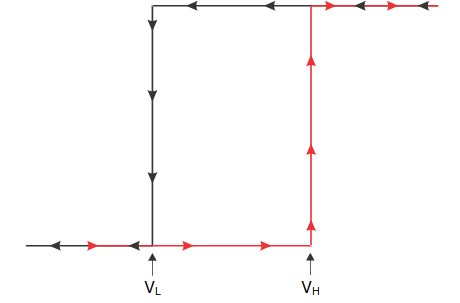
\includegraphics[width=.4\textwidth]{hysteresis}
    \caption{Comparator hysteresis}
    \label{fig:ch}
\end{figure}


We search for $V_H$, the voltage where the comparator output will transition from low to high.

$V_{TH}$ is the threshold voltage applied to the inverting input of the comparator. This is also known bias voltage.




\begin{figure}[h]
    \centering
    \begin{subfigure}[b]{0.4\textwidth}
        \centering
        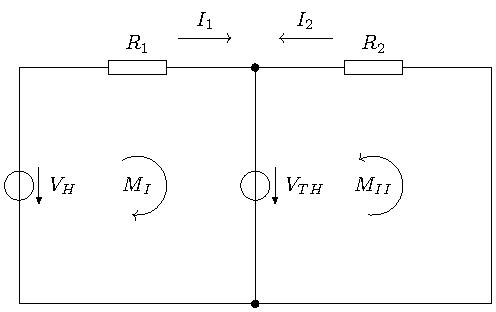
\includegraphics[width=\linewidth]{circuits/hysteresis1.pdf}
        \subcaption{KK for low-high transition}
        \label{fig:lh}
    \end{subfigure}
    \hfill
    \begin{subfigure}[b]{0.45\textwidth}
        \centering
        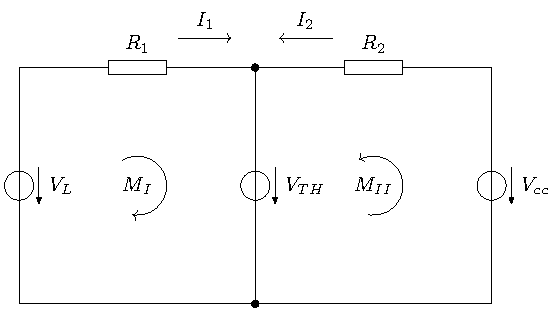
\includegraphics[width=\linewidth]{circuits/hysteresis2.pdf}
        \subcaption{KK for high-low transition}
        \label{fig:hl}
    \end{subfigure}
    \caption{Equivalent circuits for hysteresis equations}
    \label{fig:ui}
\end{figure}


Applying KKL for Fig \ref{fig:lh} gives us:



\begin{align*} \label{lh}
    V_{TH} - V_H + R_1 I_1 = 0                   \tag*{mesh {$M_I$}}    \\
    V_{TH} + R_2 I_2 = 0                         \tag*{mesh {$M_{II}$}} \\
    I_1 + I_2 = 0                                                       \\
    \Rightarrow V_{TH} = V_H \frac{R_2}{R_1 + R_2}                      \\
    \text{let $k$} = \frac{R_2}{R_1 + R_2}                              \\
    \Rightarrow V_{TH} = V_H k                           \eqnumtag\label{eqn:lh}
\end{align*}




Applying KKL for Fig \ref{fig:hl} yields:


\begin{align*} \label{hl}
    V_{TH} - V_L + R_1 I_1 = 0               \tag*{mesh {$M_I$}}                       \\
    V_{TH} - V_{cc}  + R_2 I_2 = 0                              \tag*{mesh {$M_{II}$}} \\
    I_1 + I_2 = 0                                                                      \\
    \Rightarrow  -V_L + R_1 I_1 + V_{cc} - R_2 I_2     = 0                             \\
    \Rightarrow -V_L + V_{cc} -  I_2 (R_1 + R_2)       = 0                             \\
    \Rightarrow I_2 =  \frac{V_{cc} - V_L}{R_1 + R_2}                                  \\
    \text{let $k$} = \frac{R_2}{R_1 + R_2}                                             \\
    \Rightarrow V_{TH} =  V_{cc}(1 - k) + V_L k              \eqnumtag\label{eqn:hl}
\end{align*}


With eq. \ref{eqn:lh} and \ref{eqn:hl} we must now select values for $R_1$, $R_2$ and $V_{TH}$. In practice, these values
are not real numbers but must be chosen from a finite set of available components. In addition, at least three different
circuit configurations for setting $V_{TH}$ are possible:

\begin{itemize}
    \item a basic voltage divider as show in (SBOA313A). The trade-off here is that larger resistors introduce more noise and
          smaller resistors increase power consumption. Since our application is subjected to large temperature variations,
          the resistors should not only feature tight tolerances (at least 0.1 \% ) but also a low temperature coefficient.
          Such resistors are expensive.
    \item a voltage divider followed by a low noise op amp in buffer configuration. This choice increases component count and
          cost.
    \item a voltage reference or voltage regulator with low temperature drift.  This reduces component count ( but not necessarily cost)
          and offers the best accuracy. The trade-off here is that only a small set of reference voltages is available as
          single component which means that eq. \ref{eqn:lh} and \ref{eqn:hl} can only be approximated.
\end{itemize}

We chose the last option since it minimizes component count. Selecting voltage regulator $U_7$ with
$V_{TH} = \SI{1.9}{V}$, $R_1 = \SI{129}{\kilo\ohm}$ and $R_2 = \SI{569}{\kilo\ohm}$
approximates the desired tripping voltages
$V_l=\qty{3.7}{\V}$ and $V_h=\qty{3.9}{\V}$ with acceptable accuracy.

This is verified with the help of a circuit simulator.



\subsubsection{Simulation the power supervisor circuit}


We use \href[]{https://www.analog.com/en/design-center/design-tools-and-calculators/ltspice-simulator.html}{LTSpice 17.1.10}.
We simulate $V_L=\qty{2.89}{\V}$ and $V_H=\qty{3.84}{\V}$. Recall that the goal was $V_L=\qty{3.0}{\V}$ and $V_H=\qty{3.9}{\V}$.
This deviation is acceptable for our application.


\begin{figure}[h]
    \centering
    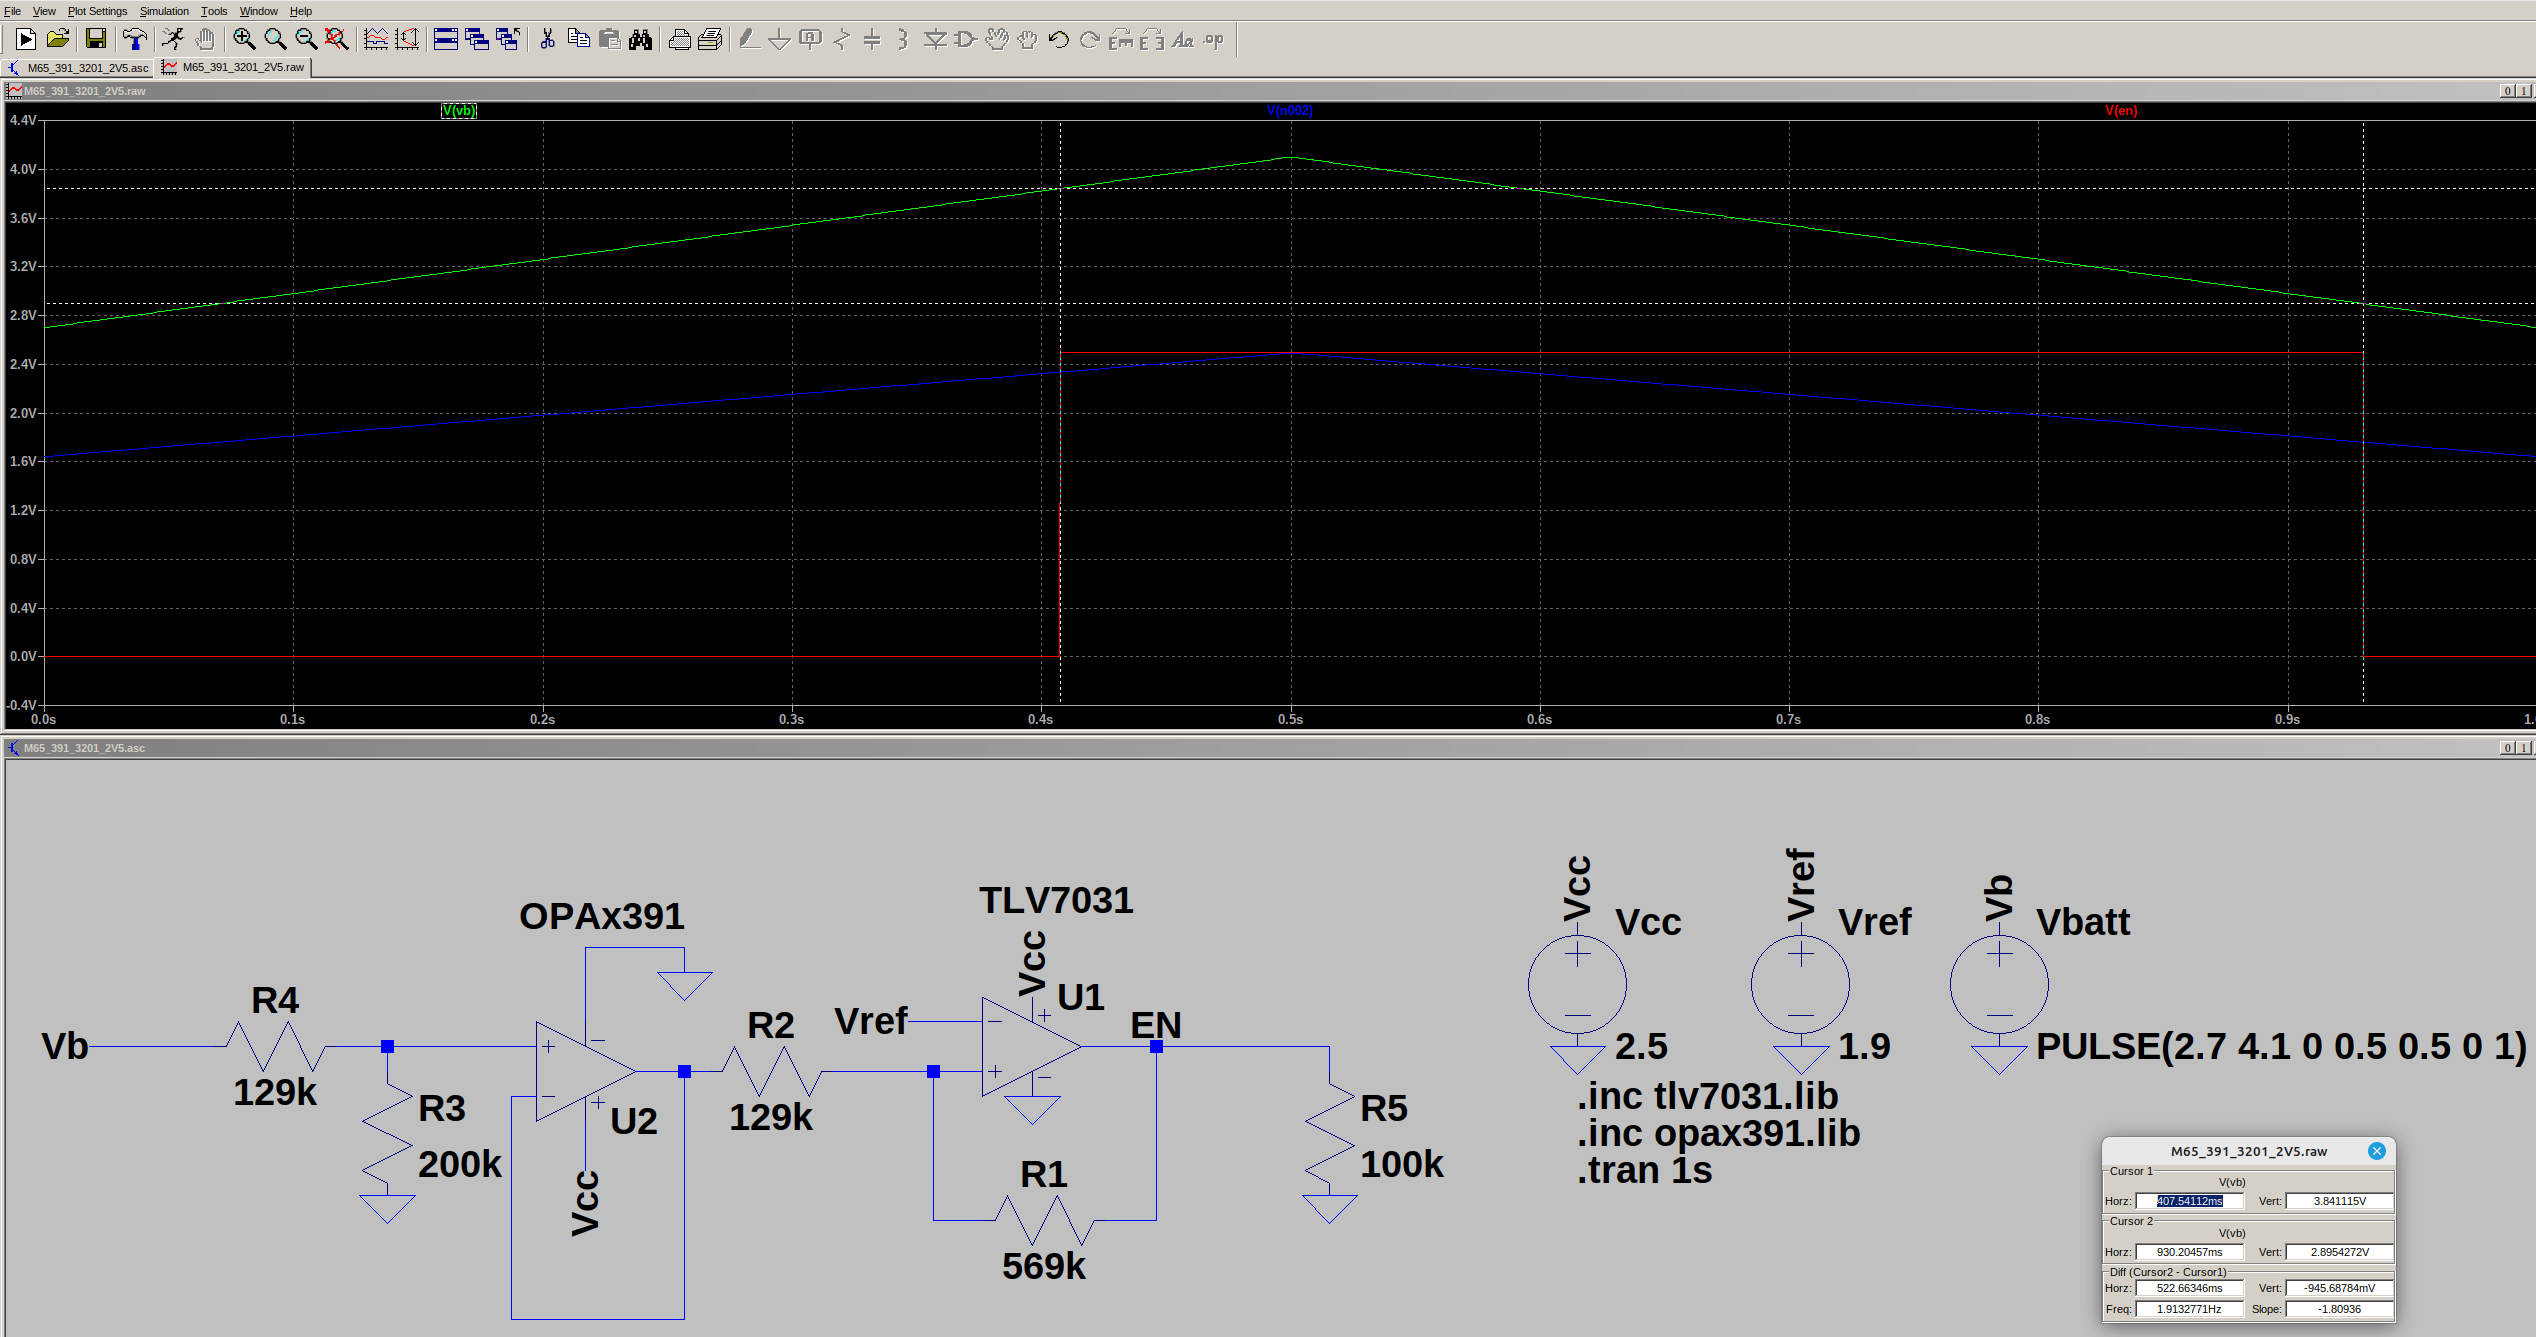
\includegraphics[width=\textwidth]{supervisor-sim}
    \caption{Power supervisor Spice simulation}
    \label{fig:sss}
\end{figure}


\clearpage

\subsection{Master Switch module (MS)}

The Master Switch module (MS) is identical to \ref{sec:SS} as far as the BOM is concerned.


\subsubsection*{Implementation}


\begin{figure}[h]
    \centering
    \includegraphics[width=0.3\textwidth]{PO/MS/MS}
    \caption{MS - schematic, see also \ref{sec:SS}}
\end{figure}

\begin{table}[H]
    \centering
    \begin{threeparttable}[b]
        \begin{tabularx}{\linewidth}{ >
                    {\hsize=.25\hsize}X >
                    {\hsize=0.5\hsize}X >
                    {\hsize=.25\hsize}X  >
                    {\hsize=.5\hsize}X >
                    {\hsize=.25\hsize}X  >
                    {\hsize=3\hsize}X
            }
                  & \multicolumn{4}{c}{Pin mapping} &                                                          \\
            \cmidrule(lr){3-6}
            Id    & Net                             & Nb. & Name             & Type            & Function      \\
            \midrule
            $U_1$ & .5V                             & 1   & VIN              & \leftharpoonup  & input         \\
            $U_1$ & \Gnd                            & 2   & \texttt{GND}     & \Gnd            &               \\
            $U_1$ & .EMS                            & 3   & \texttt{EN/UVLO} & \rightharpoonup & switch enable \\
            $U_1$ & .V\textsubscript{\mu M}         & 6   & \texttt{VOUT}    & \rightharpoonup & output        \\
        \end{tabularx}
    \end{threeparttable}

\end{table}




\clearpage











